\documentclass[12pt, titlepage]{article}
\usepackage{pdflscape}
\usepackage{longtable}
\usepackage{booktabs}
\usepackage{tabularx}
\usepackage{hyperref}
\usepackage{siunitx}
\usepackage{booktabs}
\usepackage{graphicx}
\usepackage[margin=1in]{geometry}
\usepackage[table]{xcolor}
\usepackage{float}
\hypersetup{
    colorlinks=true,    % Activate colored links
    linkcolor=red,      % Color of internal links
    citecolor=blue,     % Color of citation links
    urlcolor=blue,      % Color of URL links
    filecolor=black     % Color of file links
}
\usepackage[round]{natbib}

%% Comments

\usepackage{color}

\newif\ifcomments\commentstrue %displays comments
%\newif\ifcomments\commentsfalse %so that comments do not display

\ifcomments
\newcommand{\authornote}[3]{\textcolor{#1}{[#3 ---#2]}}
\newcommand{\todo}[1]{\textcolor{red}{[TODO: #1]}}
\else
\newcommand{\authornote}[3]{}
\newcommand{\todo}[1]{}
\fi

\newcommand{\wss}[1]{\authornote{blue}{SS}{#1}} 
\newcommand{\plt}[1]{\authornote{magenta}{TPLT}{#1}} %For explanation of the template
\newcommand{\an}[1]{\authornote{cyan}{Author}{#1}}

%% Common Parts

\newcommand{\progname}{ProgName} % PUT YOUR PROGRAM NAME HERE
\newcommand{\authname}{Team \#, Team Name
\\ Student 1 name
\\ Student 2 name
\\ Student 3 name
\\ Student 4 name} % AUTHOR NAMES                  

\usepackage{hyperref}
    \hypersetup{colorlinks=true, linkcolor=blue, citecolor=blue, filecolor=blue,
                urlcolor=blue, unicode=false}
    \urlstyle{same}
                                

The purpose of reflection questions is to give you a chance to assess your own
learning and that of your group as a whole, and to find ways to improve in the
future. Reflection is an important part of the learning process.  Reflection is
also an essential component of a successful software development process.  

Reflections are most interesting and useful when they're honest, even if the
stories they tell are imperfect. You will be marked based on your depth of
thought and analysis, and not based on the content of the reflections
themselves. Thus, for full marks we encourage you to answer openly and honestly
and to avoid simply writing ``what you think the evaluator wants to hear.''

Please answer the following questions.  Some questions can be answered on the
team level, but where appropriate, each team member should write their own
response:


\begin{document}

\title{Verification and Validation Report: \progname} 
\author{\authname}
\date{\today}
	
\maketitle

\pagenumbering{roman}

\section{Revision History}
\begin{tabularx}{\textwidth}{p{3cm}p{2cm}X}
\toprule {\bf Date} & {\bf Version} & {\bf Notes}\\
\midrule
April 02 & 1.0 & Initialized by Nanthan\\

\bottomrule
\end{tabularx}


\newpage
\tableofcontents
\listoftables %if appropriate
\listoffigures %if appropriate

\section{Disclaimer}
This document has been created following the guidance of this \href{https://github.com/smiths/capTemplate/blob/main/docs/Extras/NormansPrinciples/Expectations.md}{markdown guide}. We have list all principles for 5 pages in total, which include a mix of pros and cons per principles.

\section{Norman Principles Evaluation}
\newpage



\subsection{Patient List Page}

  \begin{figure}[ht!] 
    \centering
    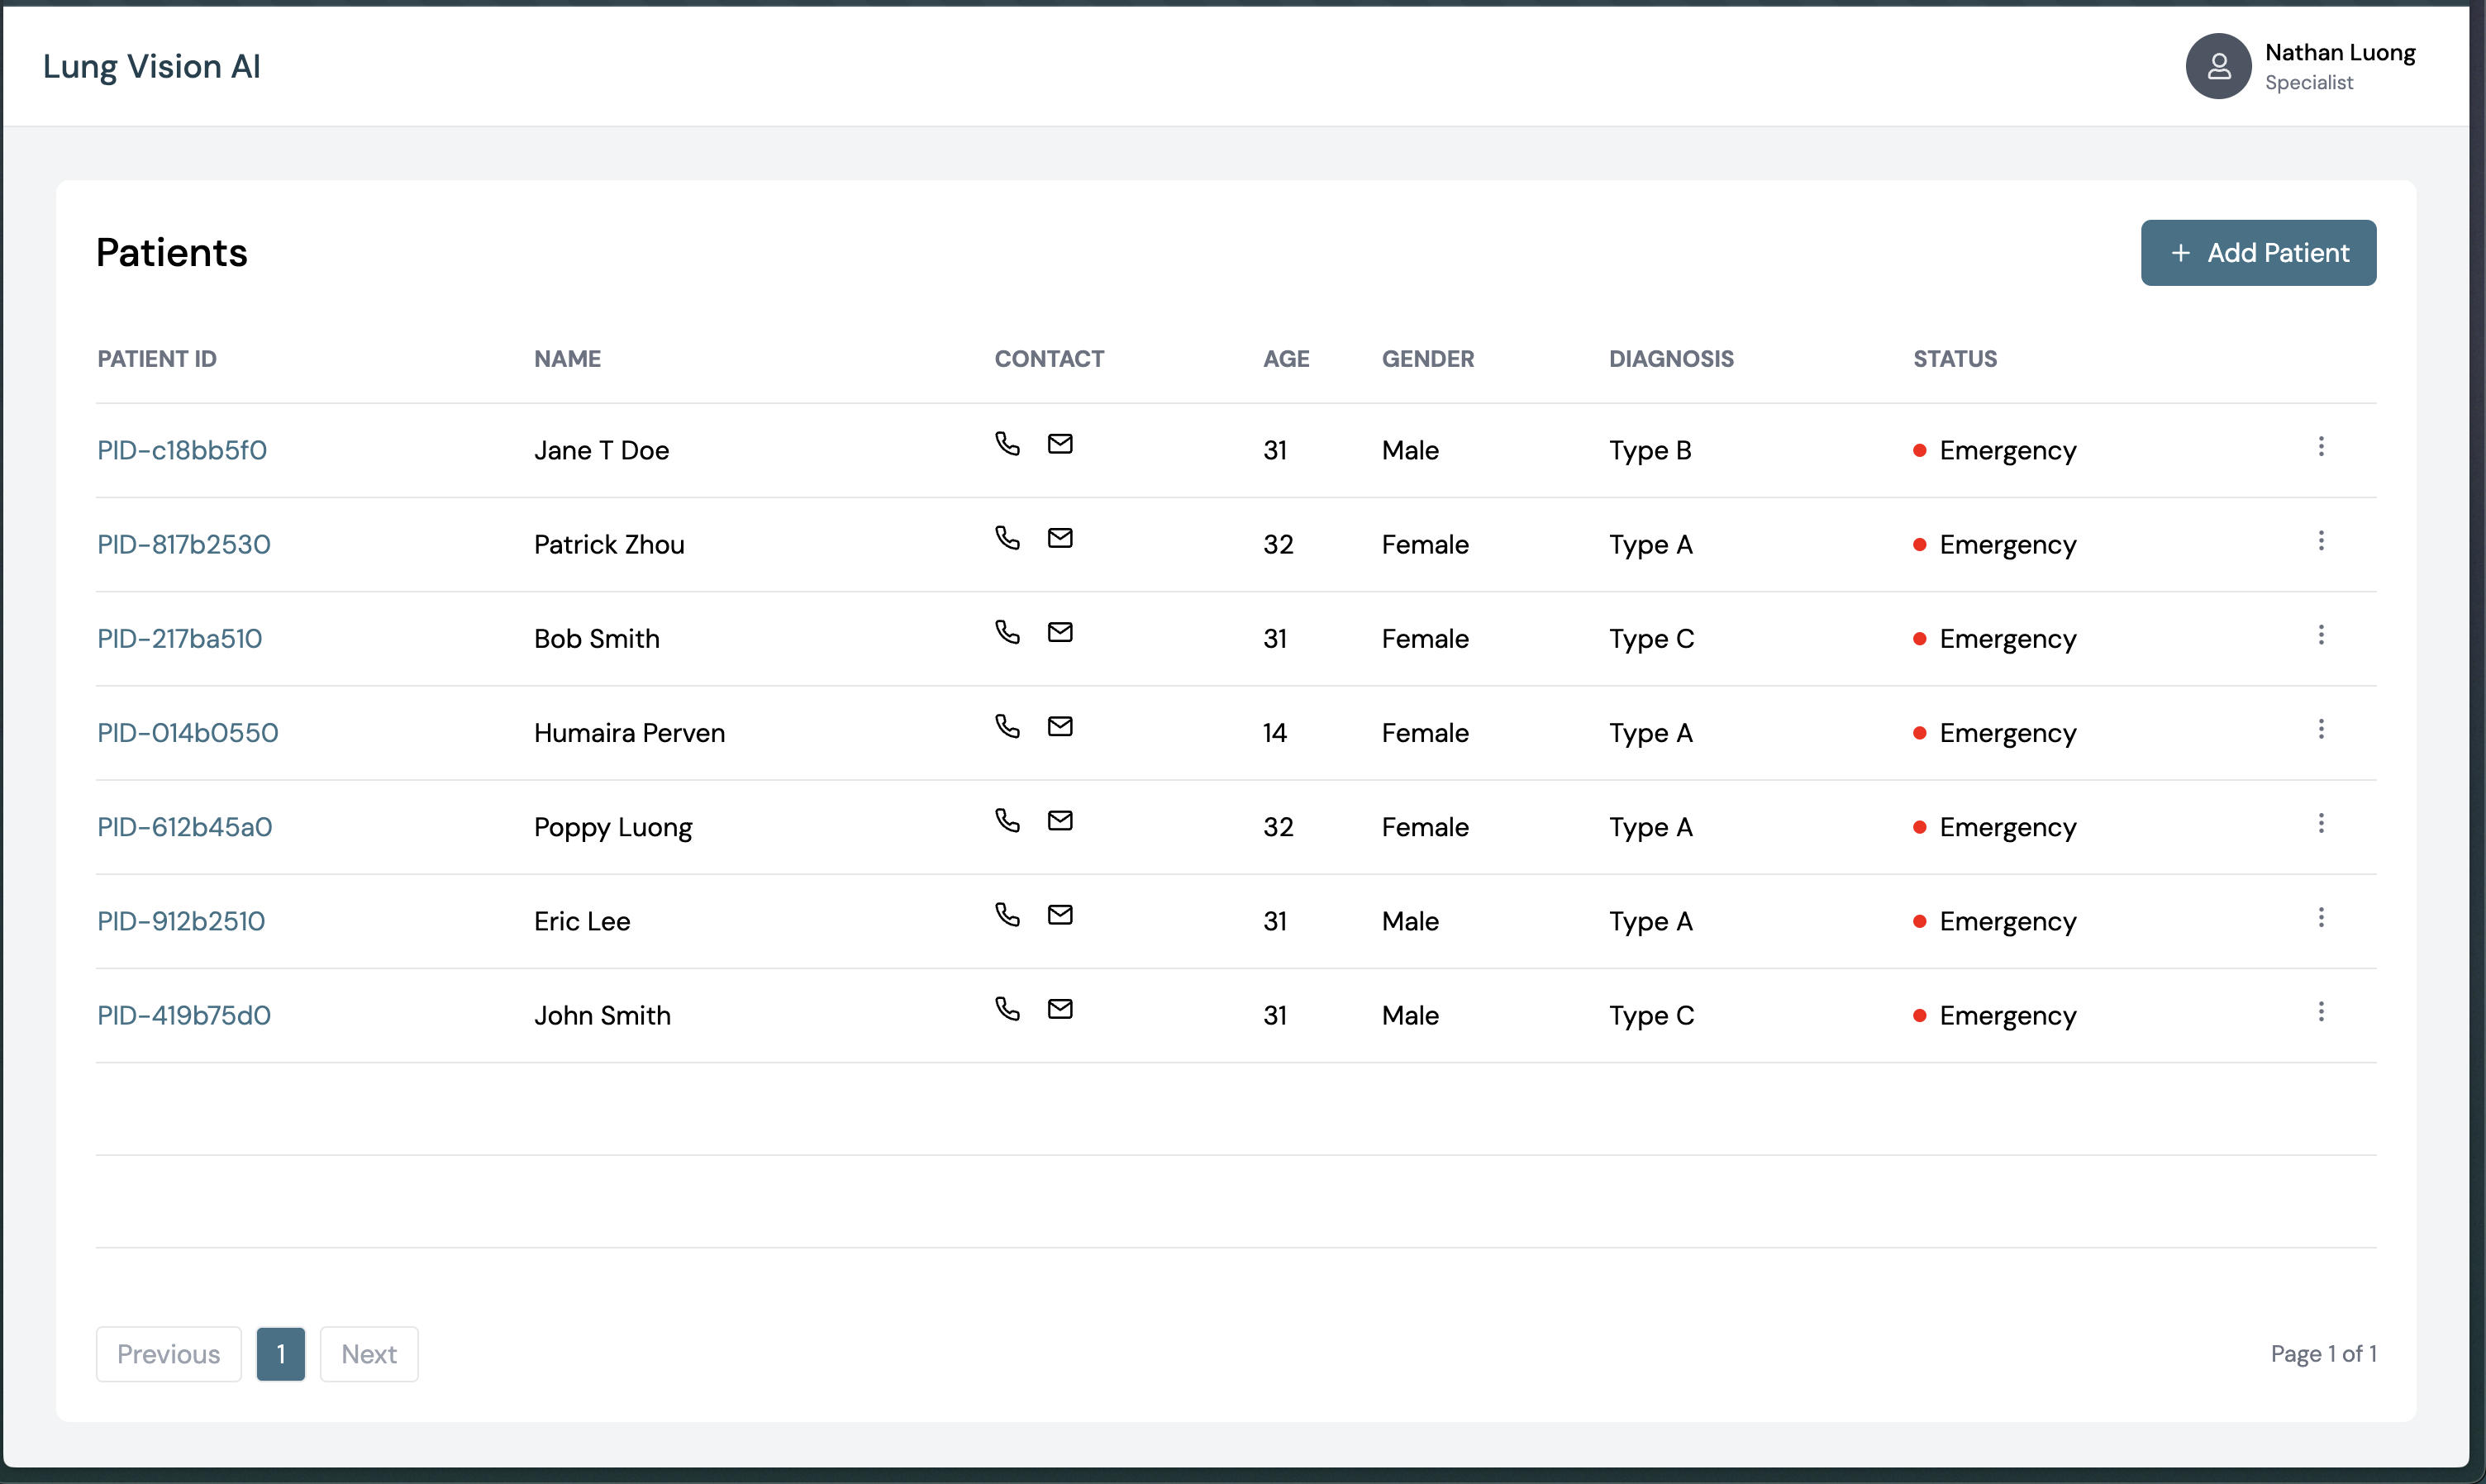
\includegraphics[scale=0.25]{../../assets/patient_list.png}
    \caption{Patient List View}
    \label{fig:patient_list}
  \end{figure}

\begin{table}[h!]
    \centering
    \rowcolors{2}{white}{white}
    \begin{tabular}{|p{2.5cm}|p{1.5cm}|p{11cm}|}
    \hline
    \rowcolor{gray!30}
    \textbf{Princicples} & \textbf{Type} & \textbf{Descriptions} \\
    \hline
    \textbf{Visibility} & Pros & Important data are too hard to see due to the small font-size and large white spaces. To improve readability, font-size should be increased.\\
    \hline
    \textbf{Feedback} & Pros & The row highlight provides clear visual feedback that a patient is selected.\\
    \hline
    \textbf{Consistency} & Pros & Visual style and patterns are consistent. Icons, rows, status dots — all behave predictably.\\
    \hline
    \textbf{Affordance} & Cons & When hover, the entire row change color, afford the user to click on the empty space on the row but not the patient's ID. To improve, hover effect on row should be less visible.\\
    \hline
    \textbf{Mapping} & Cons & The placement and appearance of the phone and email icons do not clearly indicate they trigger actions, unlike other static fields (name, status). To improve, they should be displayed as buttons to distinguish interactive elements. \\
    \hline
    \textbf{Constraints} & Cons & Clicking the email icon immediately redirects the user outside the app, which may lead to unintended navigation. The interface lacks a constraint to prevent this abrupt action. A confirmation pop-up or warning could serve as a soft constraint to guide user intent and prevent accidental redirection. \\

    \hline
    \end{tabular}
    \caption{Analysis of Patient List View}
\end{table}

\newpage
\subsection{Doctor Profile Page}

  \begin{figure}[ht!] 
    \centering
    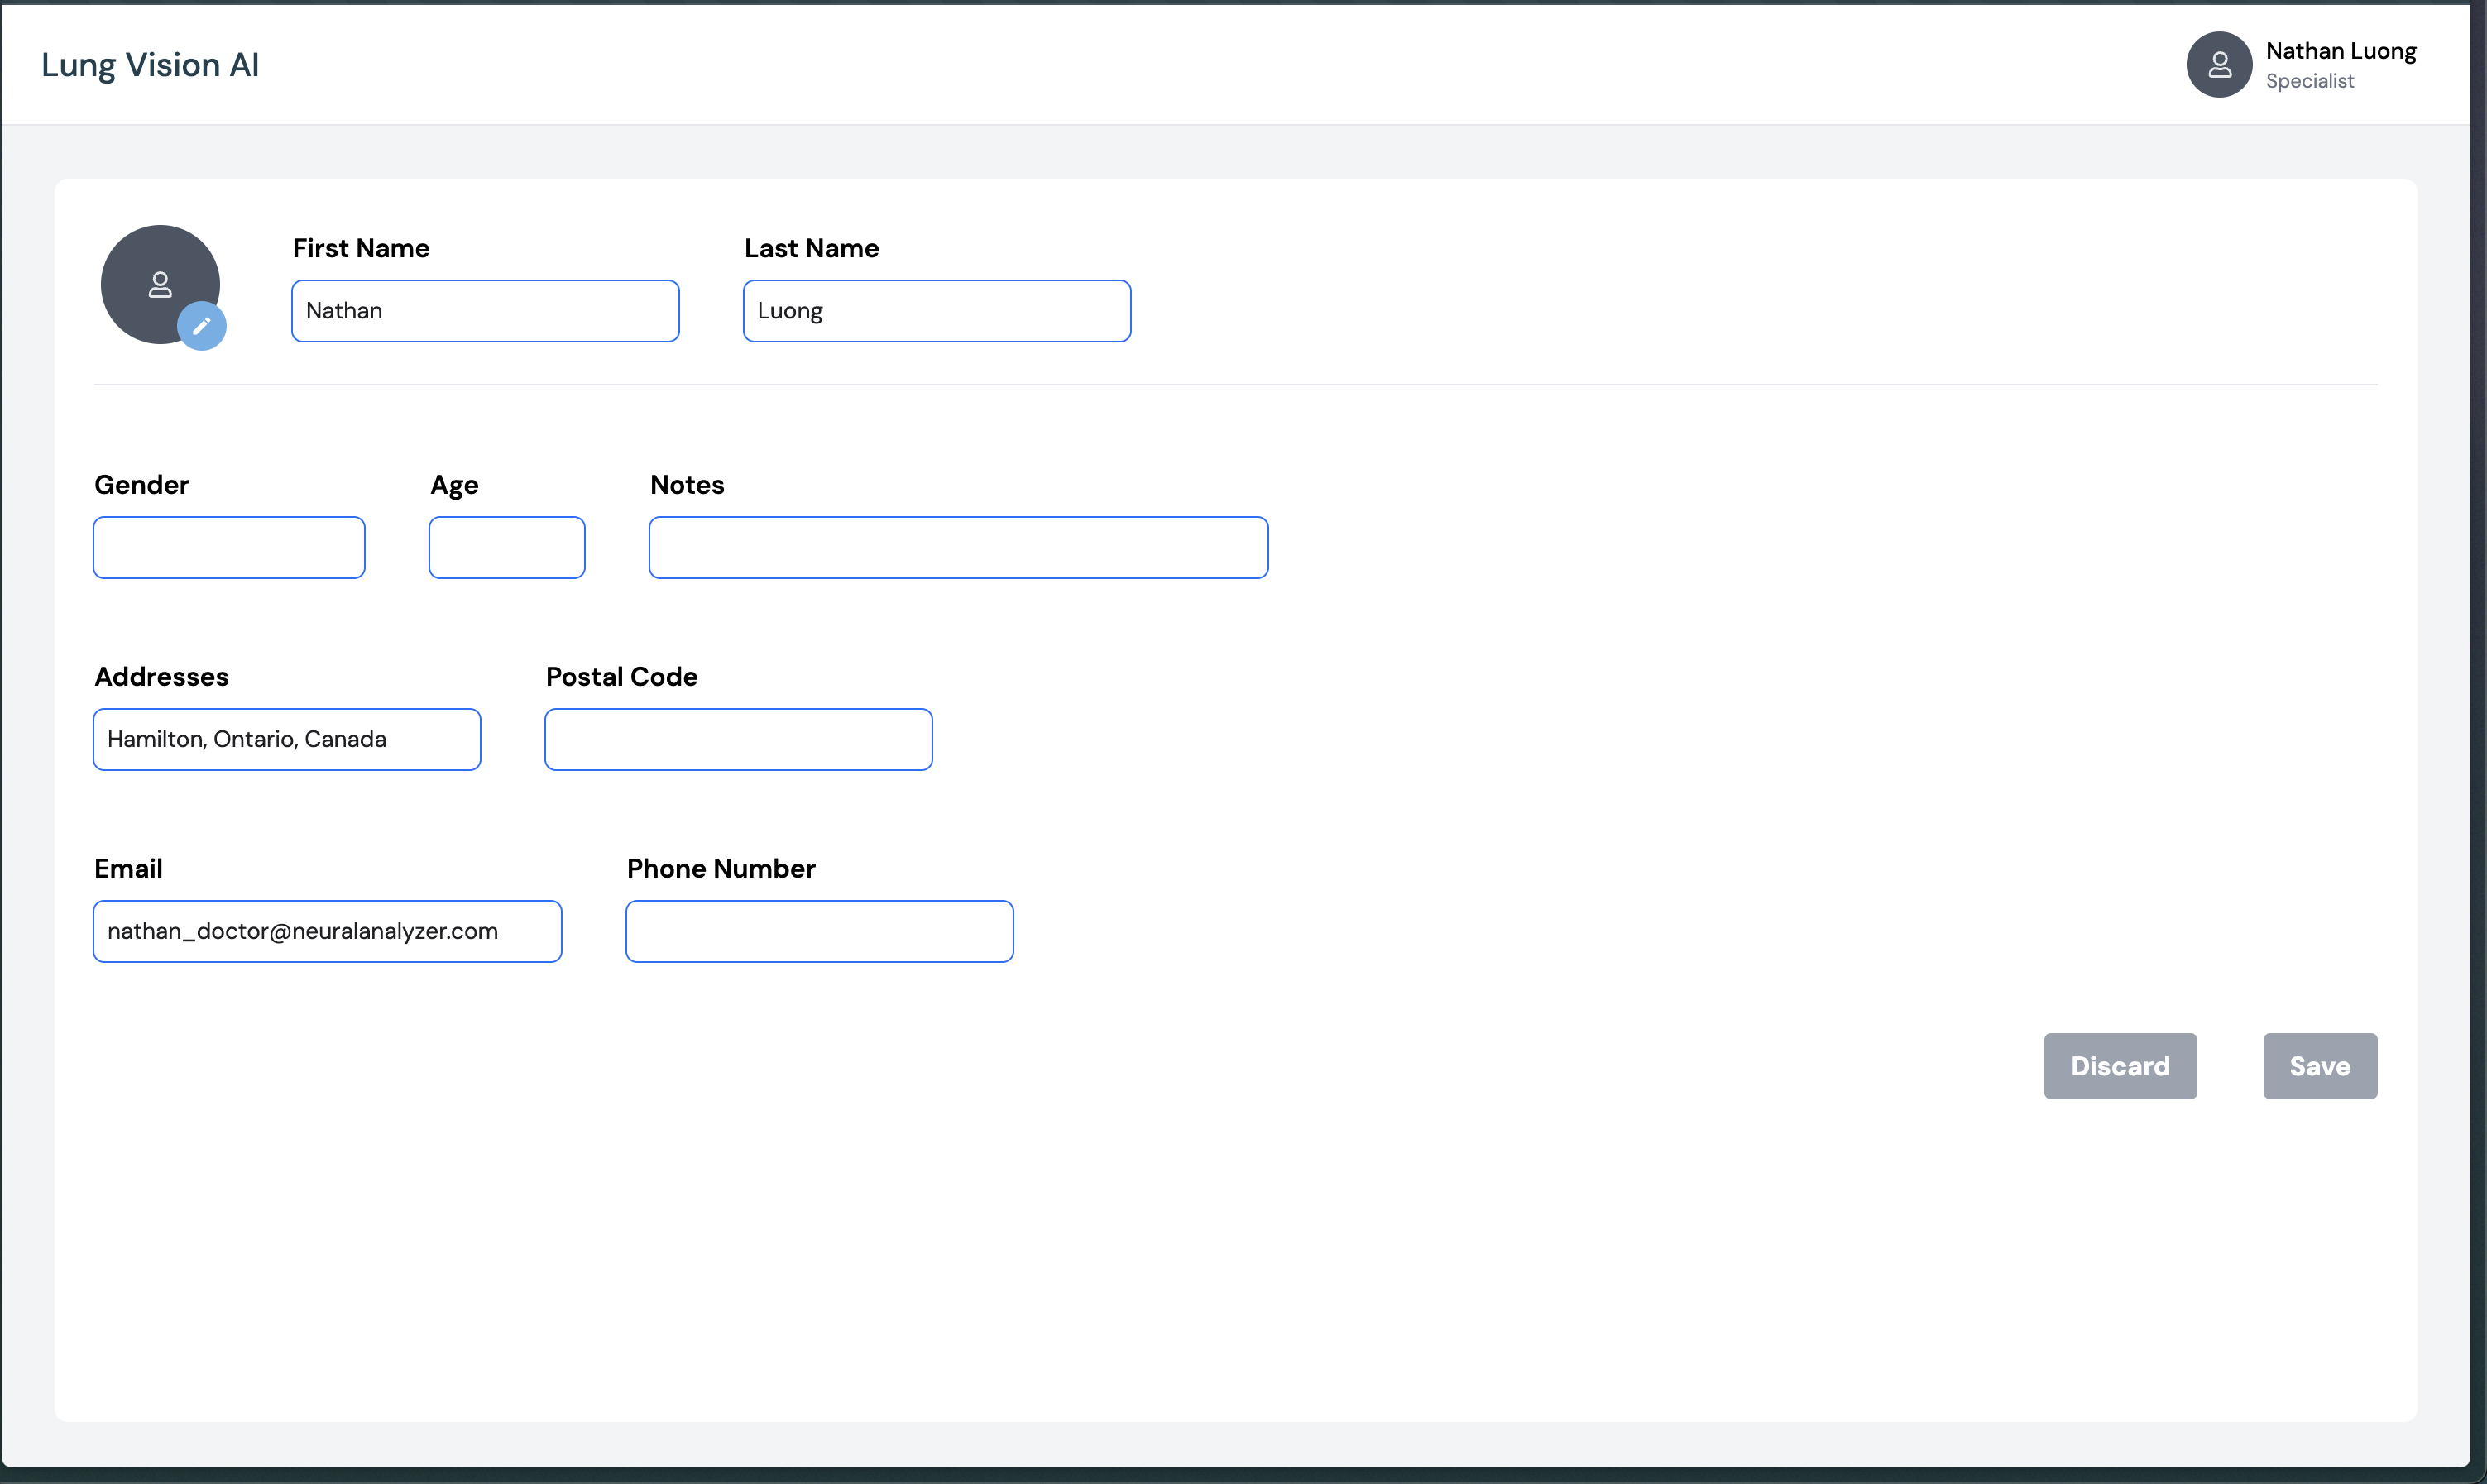
\includegraphics[scale=0.25]{../../assets/doctor_profile.png}
    \caption{Doctor Profile Page}
    \label{fig:doctor_profile_page}
  \end{figure}

\begin{table}[h!]
    \centering
    \rowcolors{2}{white}{white}
    \begin{tabular}{|p{2.5cm}|p{1.5cm}|p{11cm}|}
    \hline
    \rowcolor{gray!30}
    \textbf{Principles} & \textbf{Type} & \textbf{Descriptions} \\
    \hline
    \textbf{Visibility} & Pros & Labels and input fields are well-aligned and clearly indicate what information should be entered, making the interface easy to scan and fill out. \\
    \hline
    \textbf{Feedback} & Cons & There is no visible confirmation or indication that clicking “Save” or \"Discard\" was successful. To improve, information toast can display at the top to provide user feedback. \\
    \hline
    \textbf{Consistency} & Pros & Field styles, input borders, and spacing are consistently applied throughout the form, speeding up data entry. \\
    \hline
    \textbf{Affordance} & Cons & The “Save” and “Discard” buttons have similar visual weight, which could confuse users about which action is more critical. To improve, the buttons should contains additional cues (hover states, confirmations, ...) to support the user. \\
    \hline
    \textbf{Mapping} & Pros & Related fields are grouped together (e.g., name, contact, address), and button placement at the bottom aligns with common form expectations. \\
    \hline
    \textbf{Constraints} & Cons & Fields like “Phone Number” and “Postal Code” allow free text input without validation constraints. Input masks or format hints could prevent invalid entries and improve data quality. \\
    \hline
    \end{tabular}
    \caption{Analysis of Profile Edit Form Interface}
\end{table}



\newpage
\subsection{Patient Overview Page}

  \begin{figure}[ht!] 
    \centering
    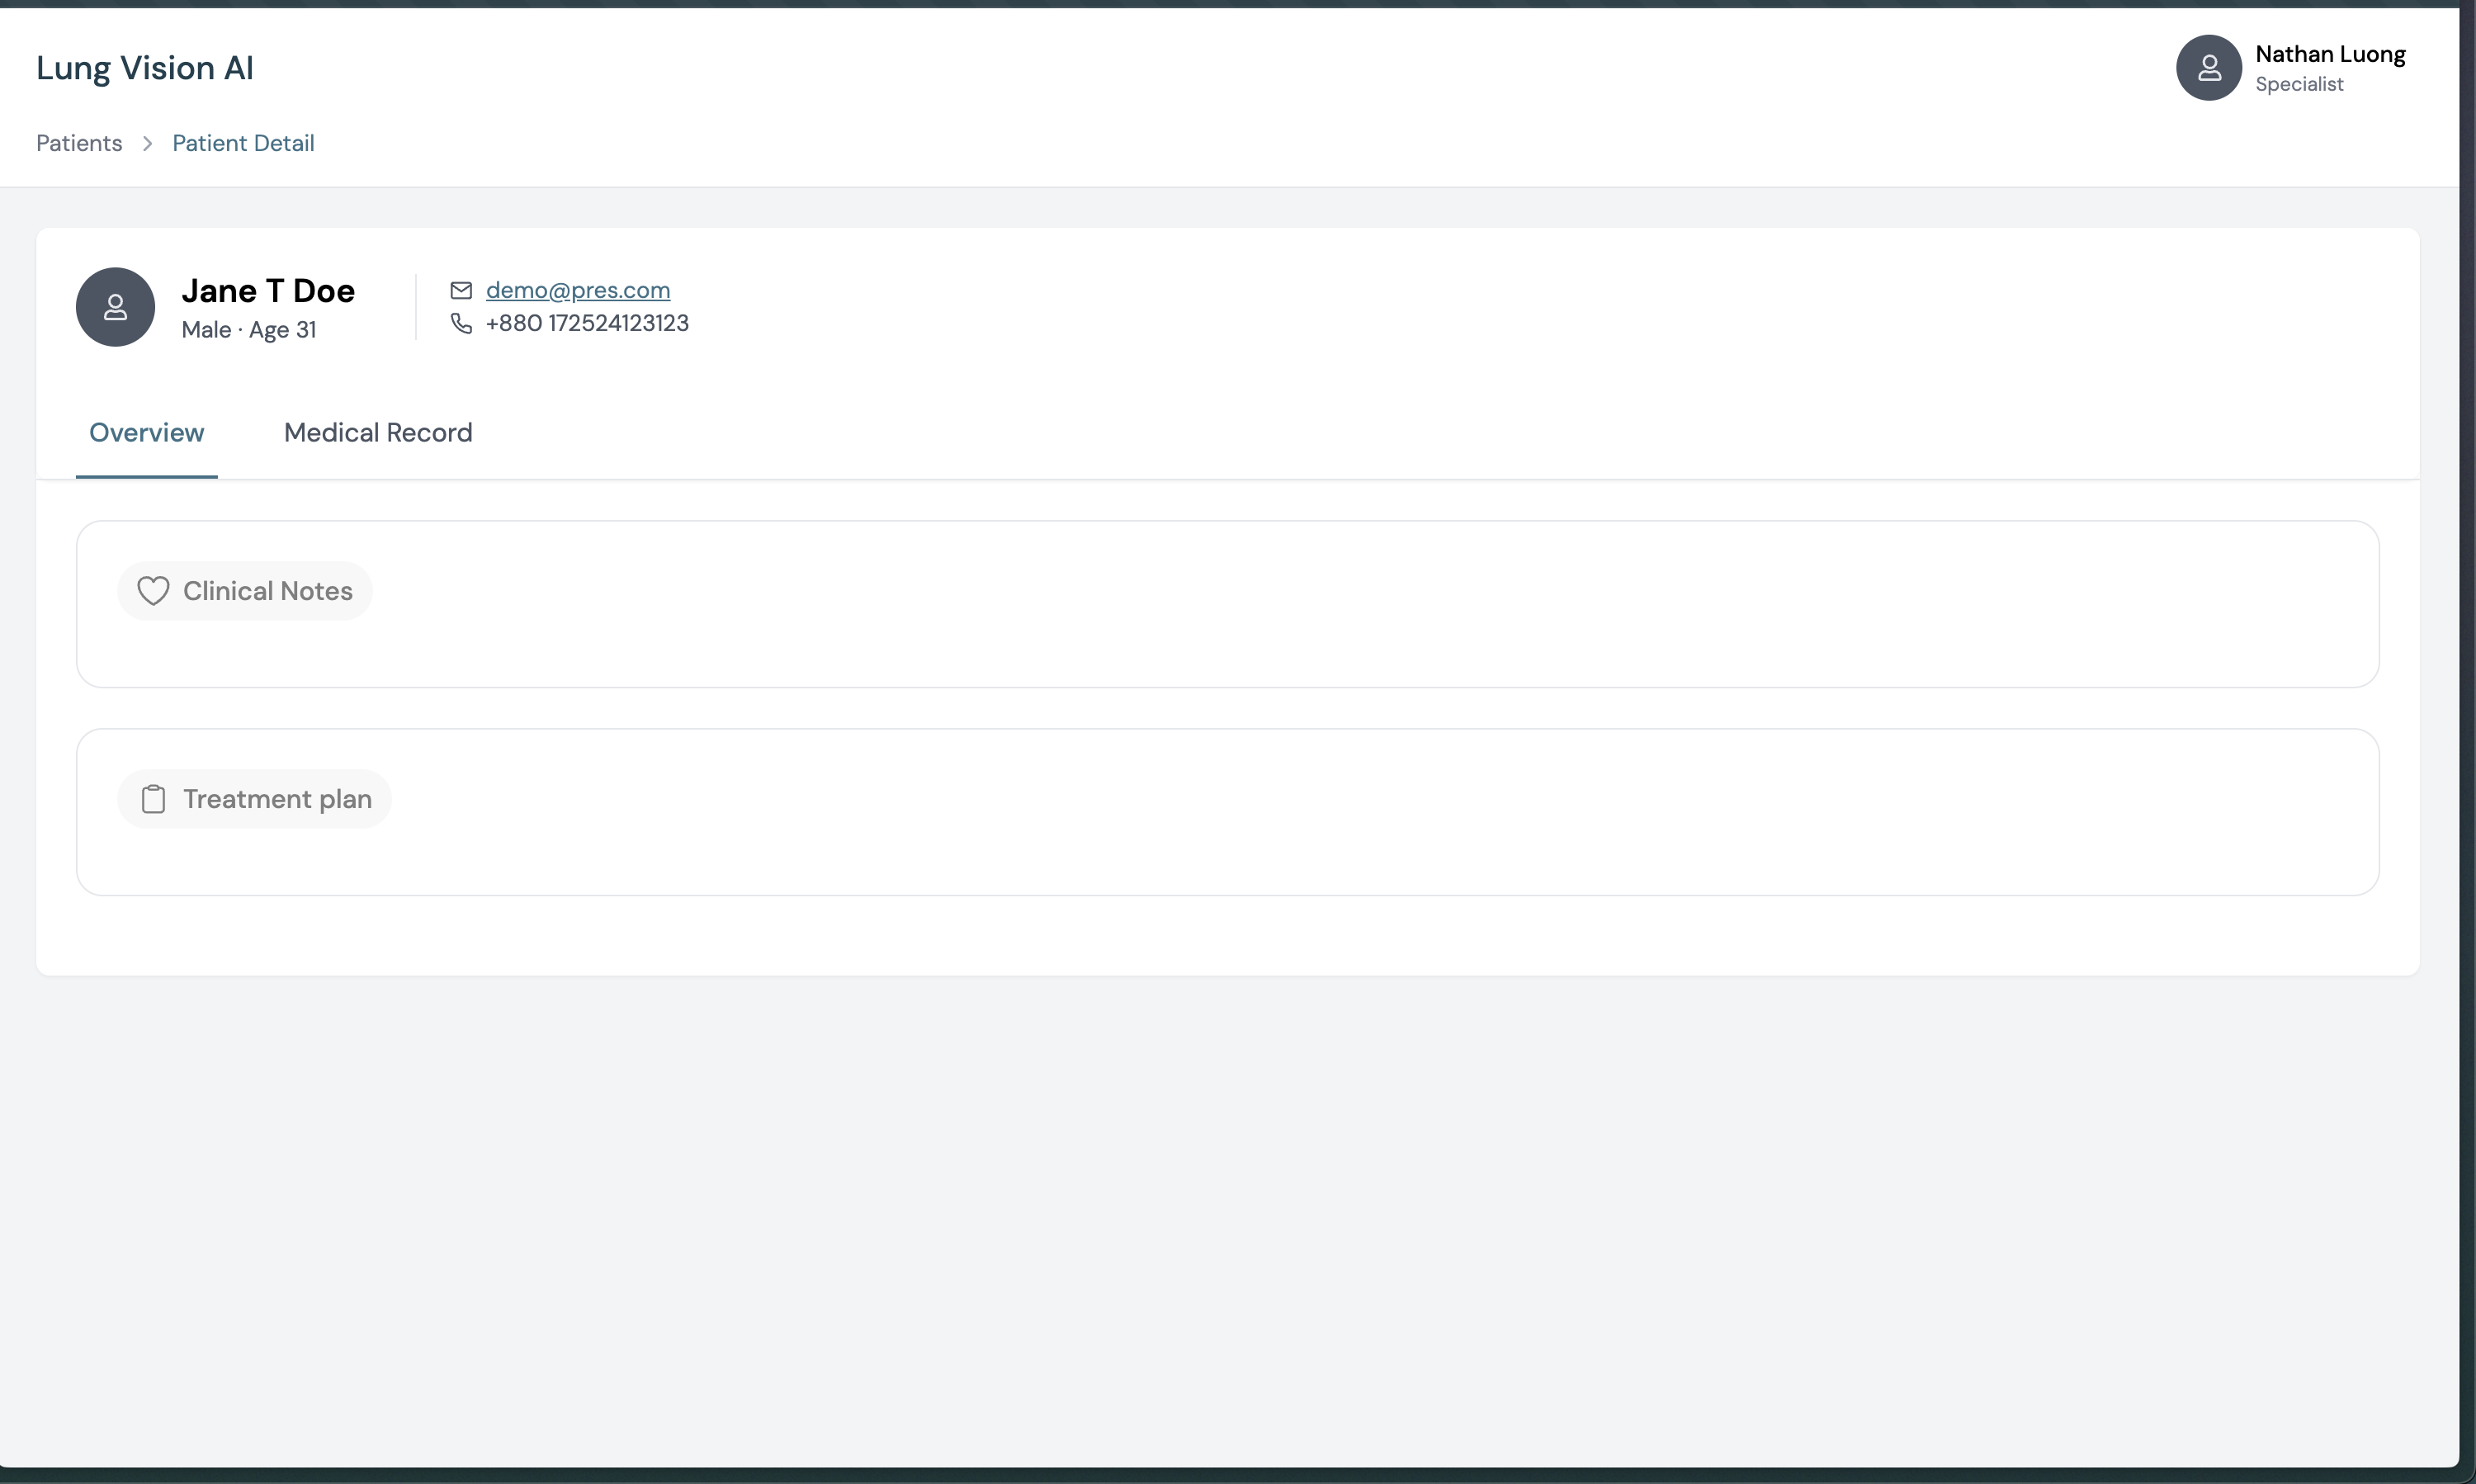
\includegraphics[scale=0.25]{../../assets/patient_overview.png}
    \caption{Patient Overview With Empty Note and Prescriptions}
    \label{fig:patient_overview}
  \end{figure}

\begin{table}[h!]
    \centering
    \rowcolors{2}{white}{white}
    \begin{tabular}{|p{2.5cm}|p{1.5cm}|p{11cm}|}
    \hline
    \rowcolor{gray!30}
    \textbf{Principles} & \textbf{Type} & \textbf{Descriptions} \\
    \hline
    \textbf{Visibility} & Pros & Key patient data such as name, age, gender, email, and phone number are prominently displayed at the top, making critical info always visible. \\
    \hline
    \textbf{Feedback} & Cons & Sections for clinical notes, or medical treatments supposed to show data from the latest visit. However, if these fields are empty, it will also show up as empty on this screen, making it un-intuitive and confusing. To improve,  the interface can show "Empty Note", or "Empty Treatment".\\
    \hline
    \textbf{Consistency} & Pros & The design language remains consistent with other screens (e.g., layout, avatar style, tab appearance), making the user experience cohesive. \\
    \hline
    \textbf{Affordance} & Cons & “Clinical Notes” and “Treatment Plan” look too similar to a button, which afford the user to click, or interact with it. To improve, a "Read Only" note can be displayed to clearify its functionality.\\
    \hline
    \textbf{Mapping} & Pros & Information on the interface is grouped logically. \\
    \hline
    \textbf{Constraints} & Pros & There are nothing to interact with on this page, user are greatly constraints to perform any action. \\
    \hline
    \end{tabular}
    \caption{Analysis of Patient Detail View}
\end{table}




\newpage
\subsection{Patient Record History Page}
  \begin{figure}[ht!] 
    \centering
    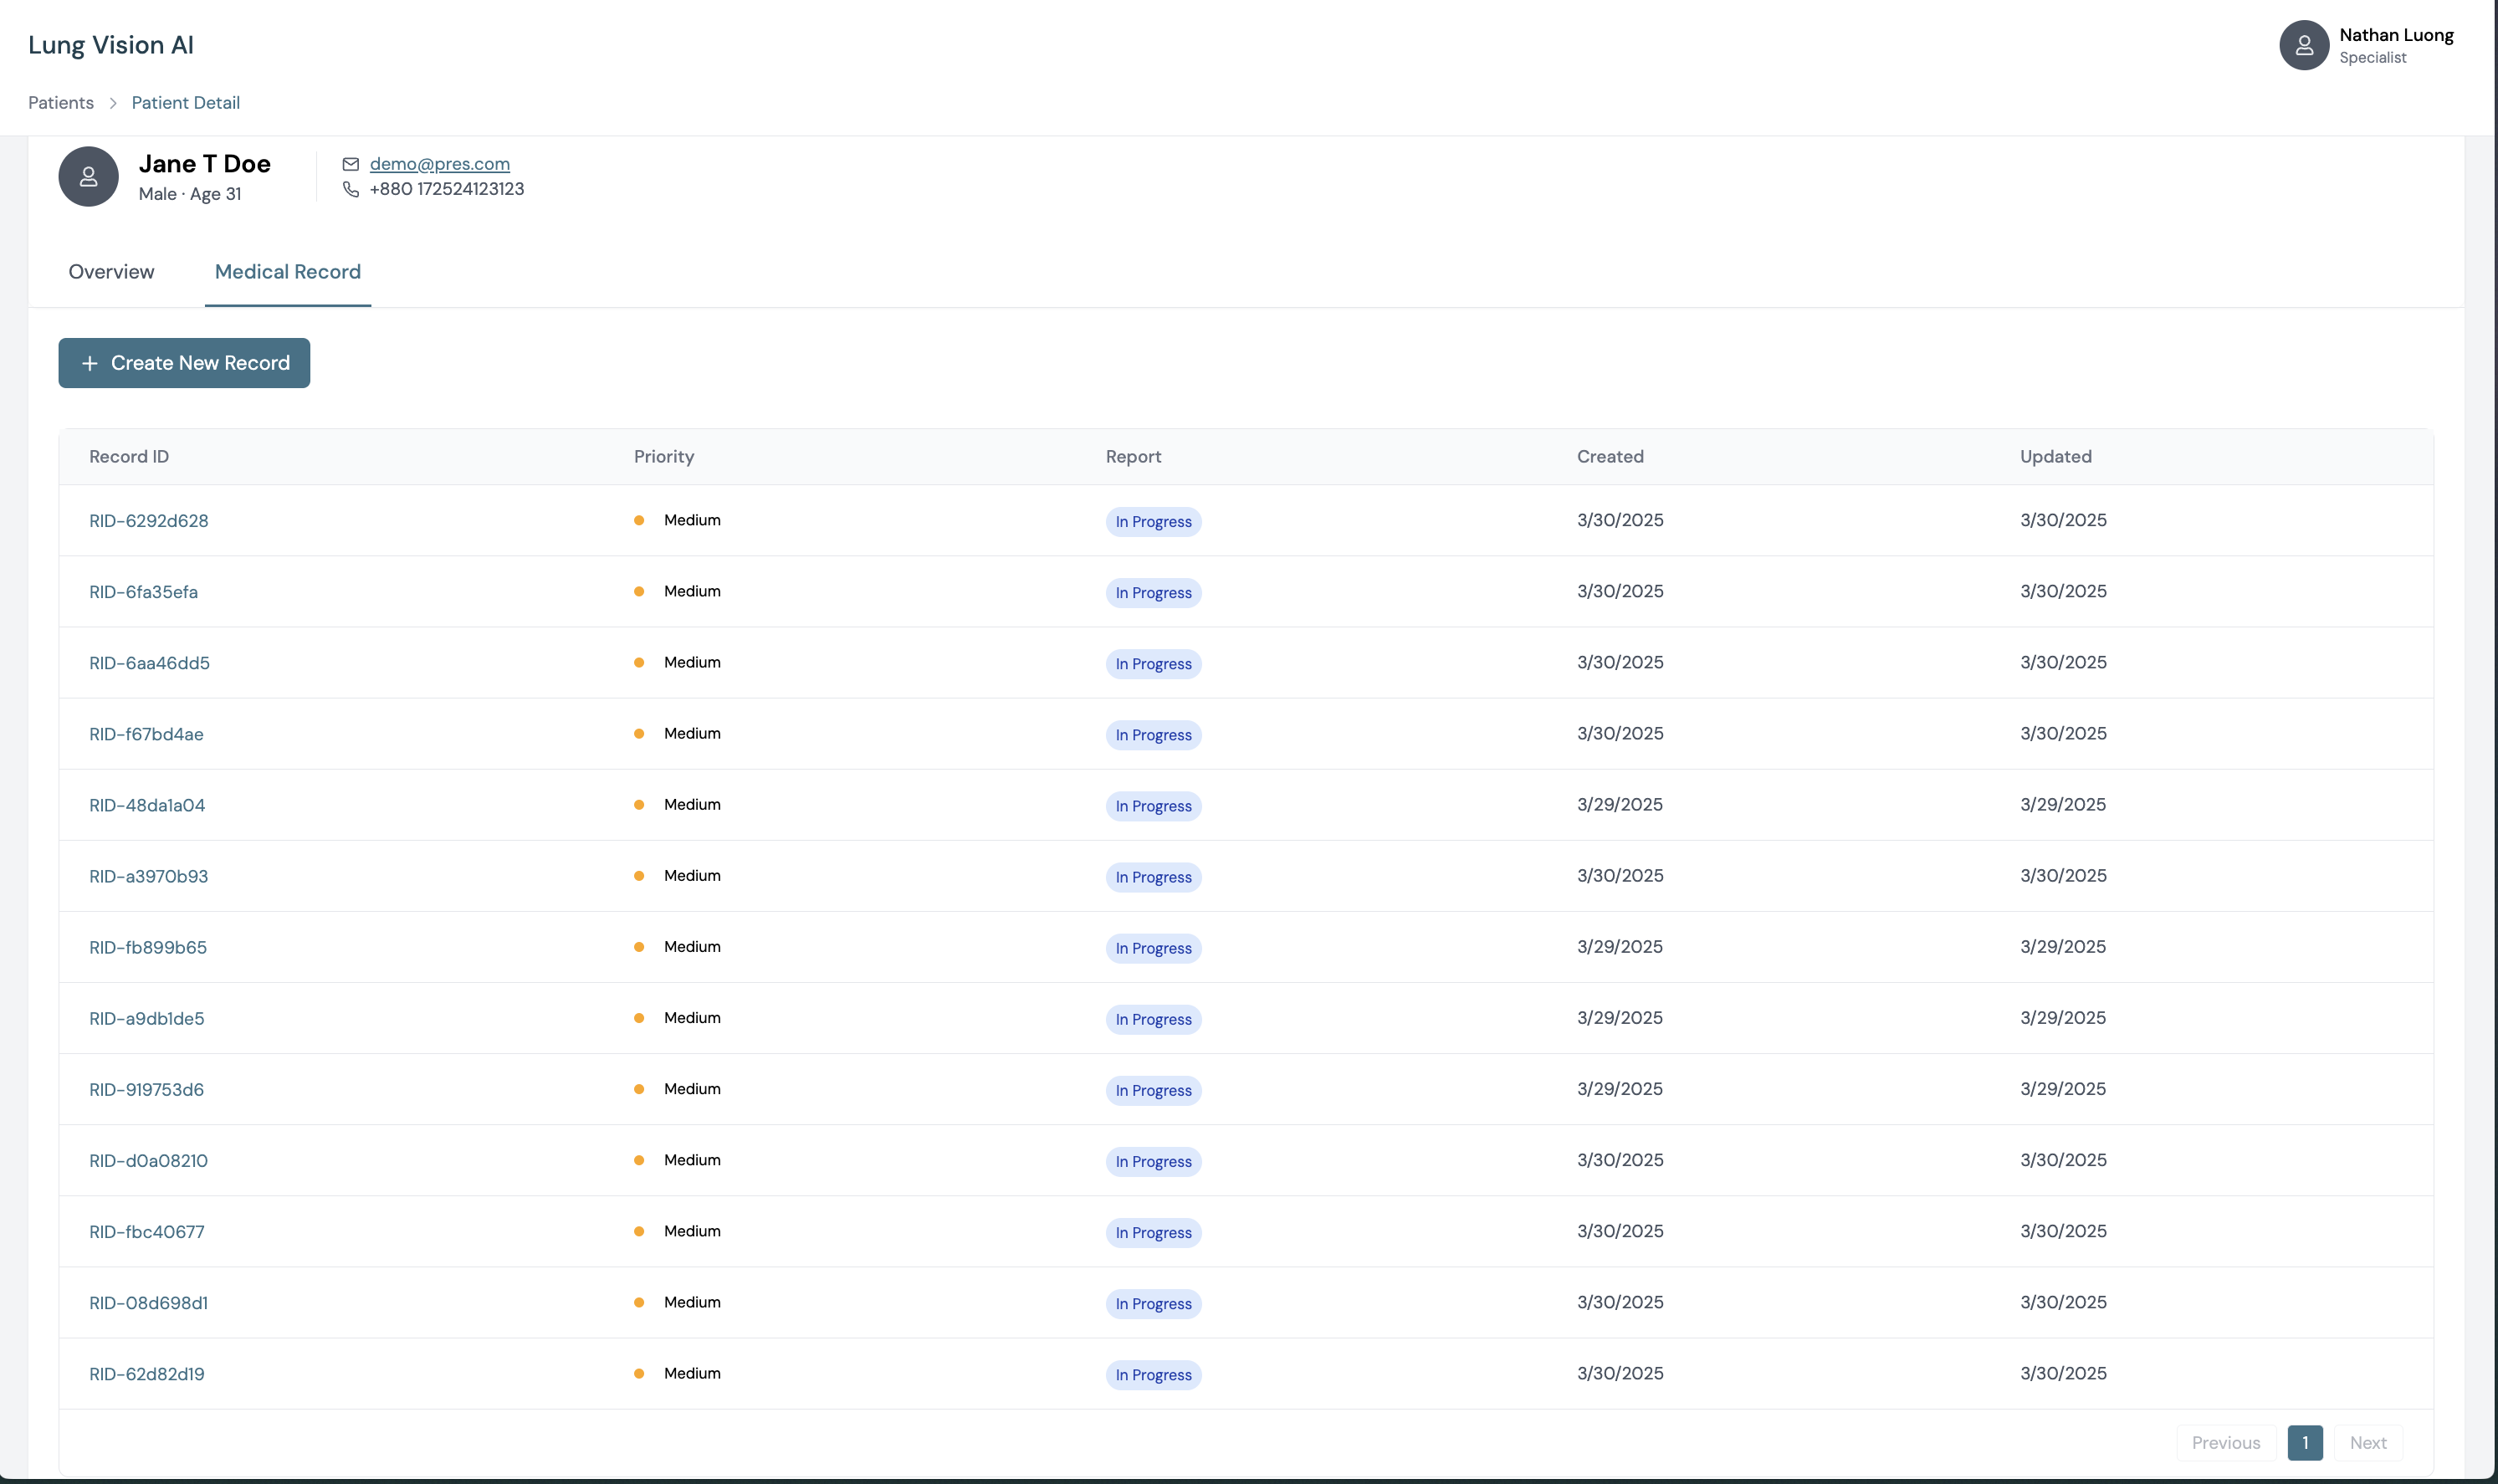
\includegraphics[scale=0.25]{../../assets/patient_records.png}
    \caption{Patient Records History}
    \label{fig:patient_records}
  \end{figure}

\begin{table}[h!]
    \centering
    \rowcolors{2}{white}{white}
    \begin{tabular}{|p{2.5cm}|p{1.5cm}|p{11cm}|}
    \hline
    \rowcolor{gray!30}
    \textbf{Principles} & \textbf{Type} & \textbf{Descriptions} \\
    \hline
    \textbf{Visibility} & Cons & Important data such as Record ID, Priority, and Status are shown on the tables, but the font-size is too small, unsuitable for time-sensitive situation such as health care. To improve, font size should be increased, and whitesapces should be minimize. \\
    \hline
    \textbf{Feedback} & Pros & Hovering effects are present for record row and Record's ID.\\
    \hline
    \textbf{Consistency} & Pros & The column structure, button styles, tag visuals (“In Progress”), and priority indicators are consistent with other views in the system. \\
    \hline
    \textbf{Affordance} & Cons & The entire row has a hovering effect afford the user to click on an empty space of the row, however this will not work. To improve, hover effect on the row should be very light and less visually appealing. \\
    \hline
    \textbf{Mapping} & Pros & The table format and content placement follow standard data table conventions. \\
    \hline
    \textbf{Constraints} & Cons & Users can click “Create New Record” regardless of system state or user role. There are no visible constraints or checks, such as disabling the button when the user lacks permission or when a max record limit is reached. This could lead to confusion or errors. \\
    \hline
    \end{tabular}
    \caption{Analysis of Medical Record Table View}
\end{table}


\newpage
\subsection{Create New Record Page}
  \begin{figure}[ht!] 
    \centering
    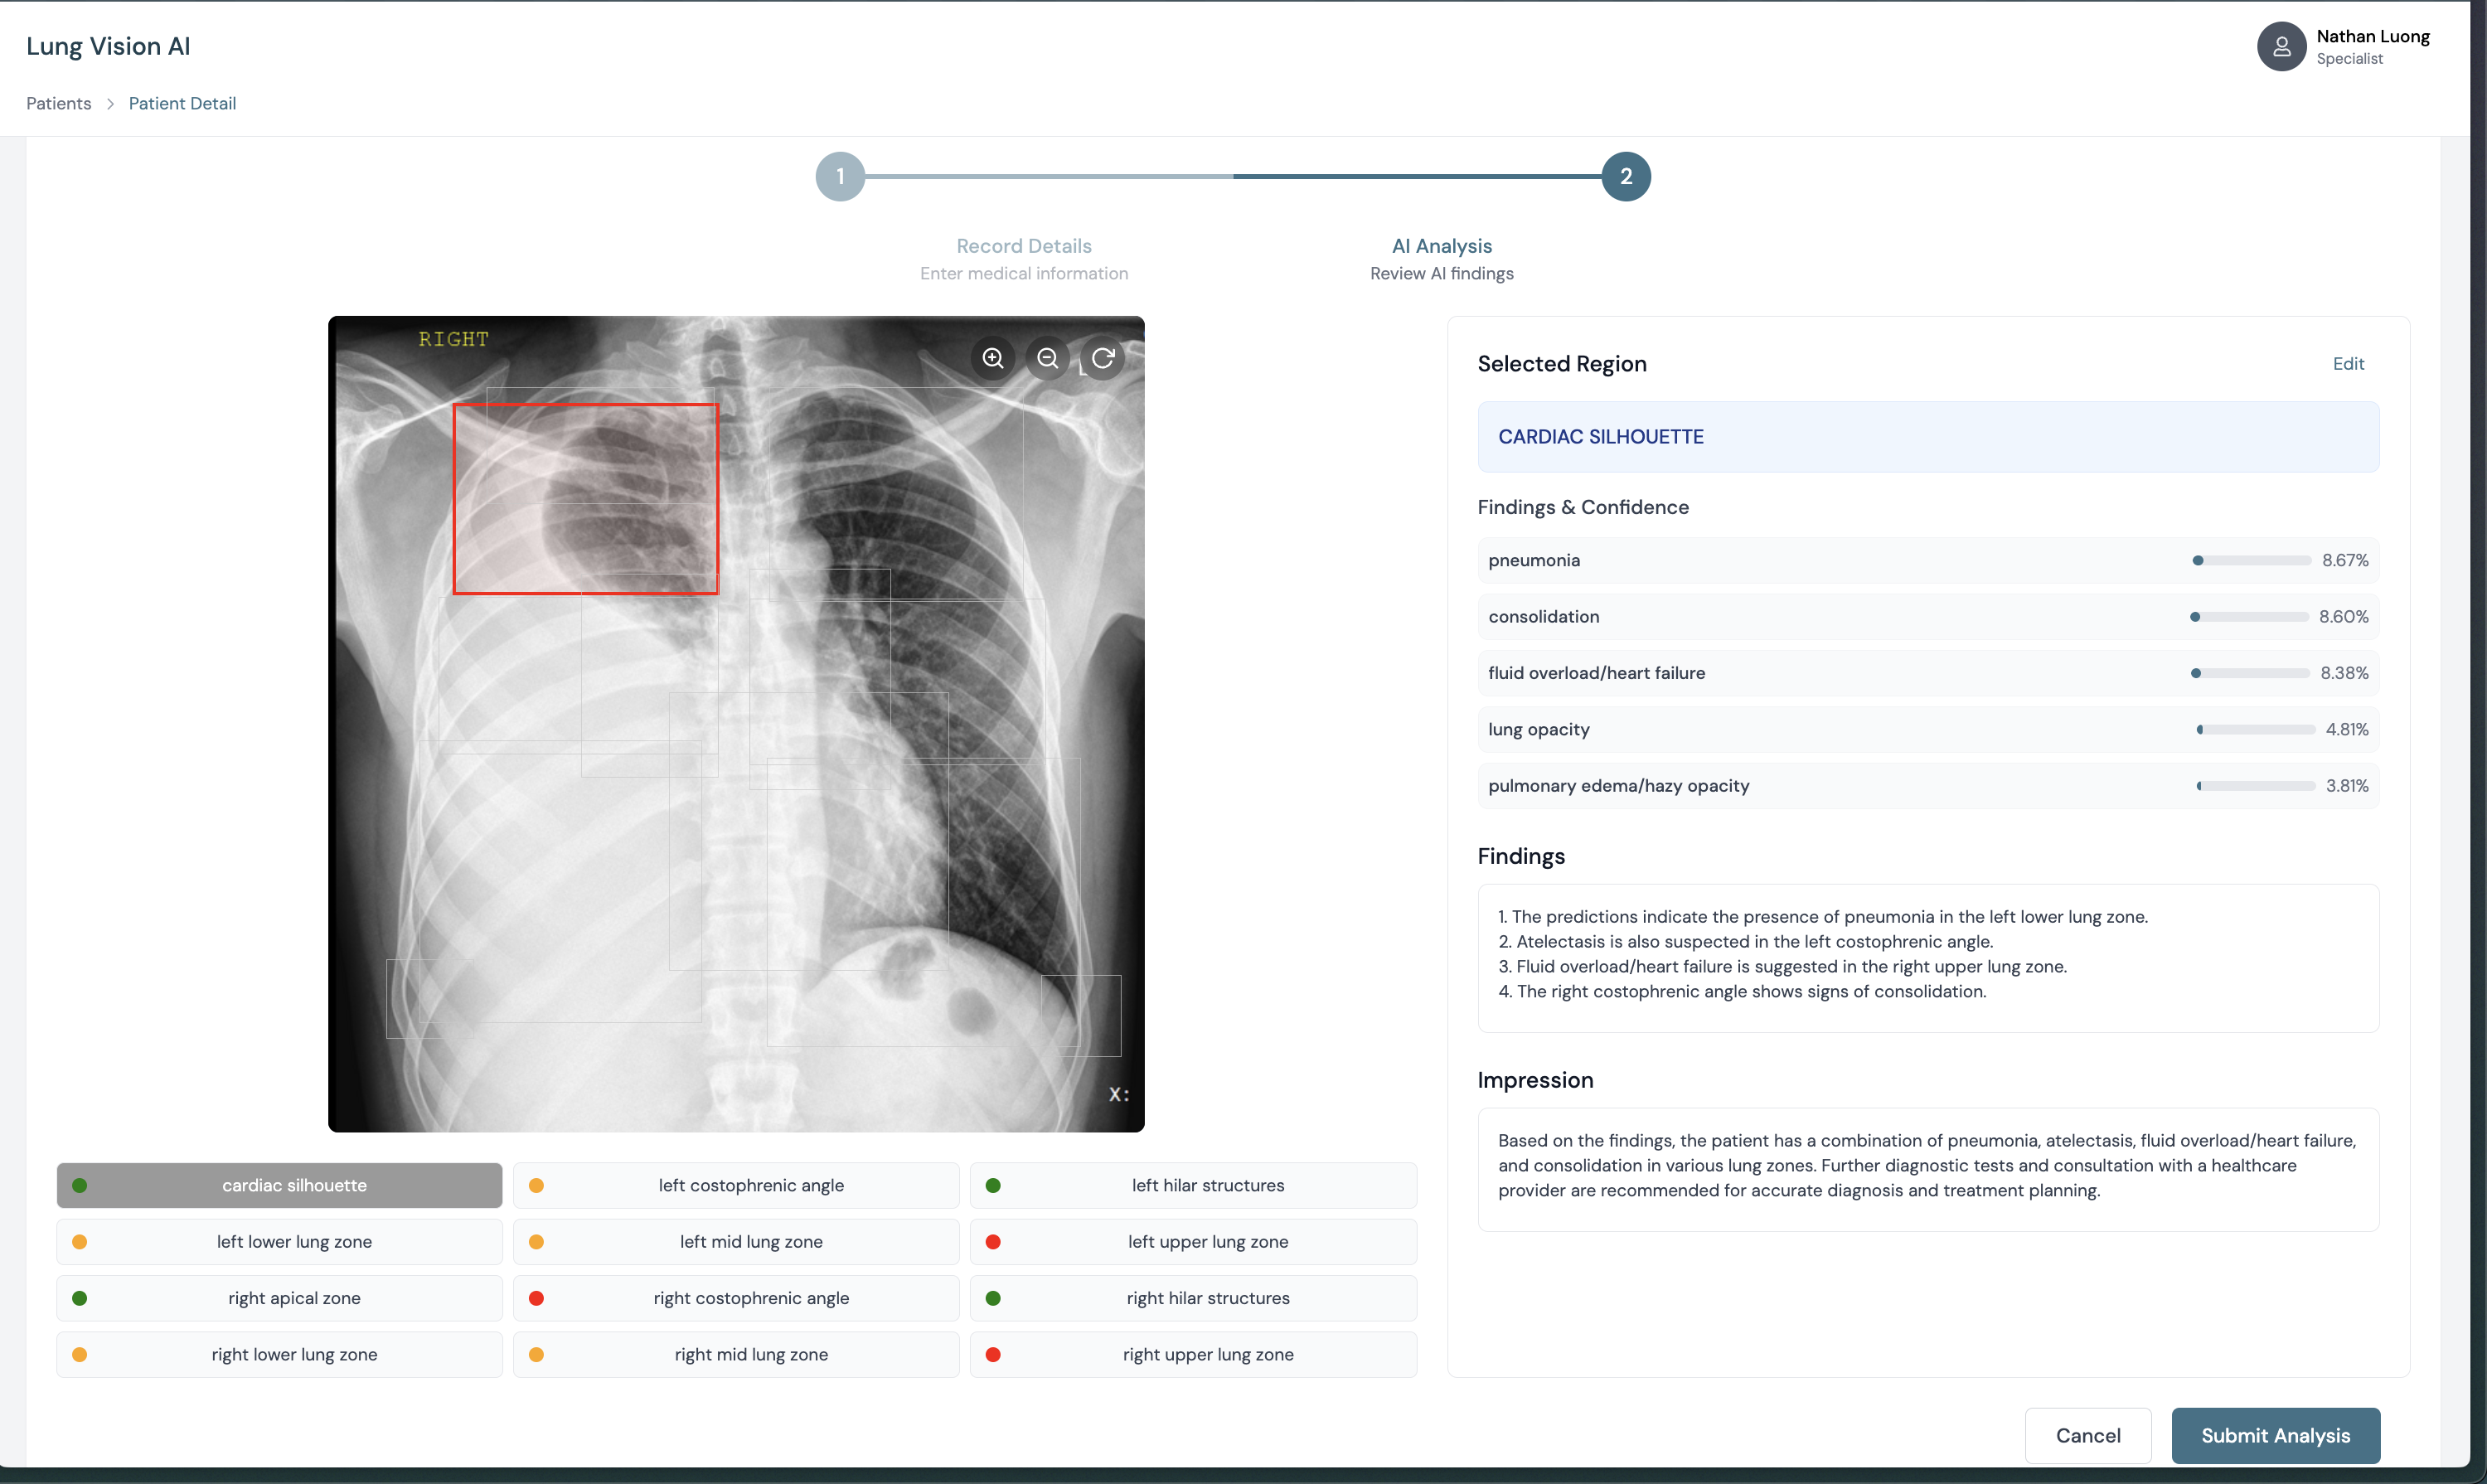
\includegraphics[scale=0.25]{../../assets/analysis_result.png}
    \caption{Machine Learning Analysis Result}
    \label{fig:new_record_4}
  \end{figure}

\begin{table}[h!]
    \centering
    \rowcolors{2}{white}{white}
    \begin{tabular}{|p{2.5cm}|p{1.5cm}|p{11cm}|}
    \hline
    \rowcolor{gray!30}
    \textbf{Principles} & \textbf{Type} & \textbf{Descriptions} \\
    \hline
    \textbf{Visibility} & Cons & There are multiple regions that user can select by clicking on the bounding boxes on the image. However, the inactive bounding boxes are extremely fainted, making it barely visible. To improve, subtle colors can be introduced on other 11 boxes to make them more visible.\\
    \hline
    \textbf{Feedback} & Pros & Clicking on a bounding box will change 3 seperate UI elements on the webpage, providing a very strong feedback that user's selection has been successful. \\
    \hline
    \textbf{Consistency} & Pros & Visual and textual elements (progress indicators, font styles, and button design) are consistent with previous screens, helping users remain oriented throughout the workflow. \\
    \hline
    \textbf{Affordance} & Cons & The lung zones at the bottom resemble buttons or tags, but it’s not visually obvious that clicking them changes the region. If they are interactive, they should have more obvious affordances like shadows, hover highlights, or tooltips. \\
    \hline
    \textbf{Mapping} & Pros & The selected region on the X-ray corresponds clearly to the section on the right panel, and the findings below map well to anatomical references. Users can make logical connections between image highlights and written data. \\
    \hline
    \textbf{Constraints} & Cons & There are way too many clickable on the screen (12 bounding boxes, 12 static buttons, Edit button, rotate, zoom buttons, etc.) User will be overwhelmed with choice which might make the UI unintuitive. To improve, there should be a help box, or video to guide user through the software.  \\
    \hline
    \end{tabular}
    \caption{Analysis of AI Analysis Screen (Medical Imaging Interface)}
\end{table}


\end{document}